\documentclass{article}

\usepackage[colorlinks]{hyperref}
\usepackage{booktabs}
\usepackage{graphicx}

\usepackage[many]{tcolorbox}

% https://tex.stackexchange.com/questions/181082/how-to-reproduce-this-box-in-tcolorbox
\newtcbox{\srcbox}{
  enhanced,
  nobeforeafter,
  tcbox raise base,
  boxrule=0.4pt,
  top=0mm,
  bottom=0mm,
  right=0mm,
  left=4mm,
  arc=1pt,
  boxsep=2pt,
  before upper={\vphantom{dlg}},
  colframe=teal!75!white,
  coltext=teal!25!black,
  colback=teal!5!white,
  overlay={
    \begin{tcbclipinterior}
      \fill[teal!75!white] (frame.south west) rectangle node[text=white,font=\sffamily\bfseries\tiny,rotate=90] {SRC} ([xshift=4mm]frame.north west);
    \end{tcbclipinterior}
  }
}

\newtcolorbox{featurebox}[1]{colback=teal!5!white,colframe=teal!75!white,title={#1}}

\newtcolorbox{codebox}{colback=teal!5!white,colframe=teal!75!white}


\newcommand{\ghsrc}[2]{\href{https://github.com/quantum-bits/capernaum/blob/development/#1}{#2}}

\newcommand{\bull}{\textsc{Bull}}
\newcommand{\caper}{\textsc{Capernaum}}
\newcommand{\cfse}{\textsc{C4se}}
\newcommand{\cli}{\textsc{Cli}}
\newcommand{\cls}{\textsc{Cls}}
\newcommand{\gh}{\textsc{GitHub}}
\newcommand{\gql}{\textsc{GraphQL}}
\newcommand{\grafana}{\textsc{Grafana}}
\newcommand{\nest}{\textsc{Nest}}
\newcommand{\nodemailer}{\textsc{Node\-mailer}}
\newcommand{\node}{\textsc{Node}}
\newcommand{\pg}{\textsc{PostgreSQL}}
\newcommand{\prometheus}{\textsc{Prometheus}}
\newcommand{\redis}{\textsc{Redis}}
\newcommand{\rest}{\textsc{Rest}ful}
\newcommand{\sio}{\textsc{Socket.IO}}
\newcommand{\ts}{\textsc{TypeScript}}
\newcommand{\tu}{TU}
\newcommand{\typeorm}{\textsc{TypeORM}}
\newcommand{\vega}{\textsc{Vega-Lite}}
\newcommand{\vuetify}{\textsc{Vuetify}}
\newcommand{\vue}{\textsc{Vue}}
\newcommand{\qual}{\textsc{Qualtrics}}

\title{\caper{} Architecture}
\author{Dr.\ Tom Nurkkala}

\begin{document}
\maketitle

\section{Introduction}
\label{sec:introduction}

\caper{} is a web-based system
that gathers responses to designated surveys taken at \href{https://www.qualtrics.com/}{\qual}.
When notified of a completed survey by a \qual{} web hook,
\caper{}
downloads the survey response
to its \href{https://www.postgresql.org/}{\pg{}} relational database
using the
\href{https://api.qualtrics.com/}{\qual{} \rest{} API}.
\caper{} then
analyzes the response and
prepares a personalized analysis for the respondent:
a \LaTeX-formatted PDF containing both a text commentary
and graphical visualizations of results.
Finally, \caper{}
emails the PDF to the survey respondent.
Figure~\ref{fig:features} highlights additional
key features of the \caper{} architecture.

\begin{figure}
  \centering
  \begin{cbox}{Key features of \caper}
    \begin{enumerate}
    \item Administrative and registration apps implemented using
      the \href{https://vuejs.org/}{\vue{}} framework and
      the \href{https://vuetifyjs.com/}{\vuetify} UI toolkit.
    \item Server software uses
      \href{https://nestjs.com/}{\nest} server-side framework
      running on \href{https://nodejs.org/}{\node}.
    \item Implemented entirely in \href{https://www.typescriptlang.org/}{\ts}.
    \item \href{https://graphql.org/}{\gql{}} API
      federates access to both relational data and an external \rest{} API.
      Uses \href{https://www.apollographql.com/}{Apollo \gql}.
    \item Push notification to administrative application
      using \href{https://socket.io/}{\sio}.
    \item Distributed job queuing system
      using \href{https://www.npmjs.com/package/bull}{\bull}
      and \href{https://redis.io/}{\redis}.
    \item Command line interface (\cli) for administration, fixture loading, and testing.
    \item Production performance monitoring using \href{https://prometheus.io/}{\prometheus}.
      Reporting and visualization via \href{https://grafana.com/grafana/}{\grafana}.
    \item Data persistence uses
      \href{https://typeorm.io/}{\typeorm} object-relational mapper
      backed by a 
      \href{https://www.postgresql.org/}{\pg{}} relational database.
    \item Report generation using \href{https://www.latex-project.org/}{\LaTeX} for typesetting
      and \href{https://vega.github.io/vega-lite/}{\vega} to render charts.
      Reports delivered to survey respondents using \href{https://nodemailer.com/}{\nodemailer}.
    \item Integrated with
      \href{https://www.qualtrics.com/}{\qual} survey platform
      using inbound web hooks and
      \href{https://api.qualtrics.com/}{\rest{} API}.
    \item Fully open source on \href{https://github.com/quantum-bits/capernaum.git}{\gh}.
    \end{enumerate}
  \end{cbox}
  \caption{Key features of the \caper{} architecture.}
  \label{fig:features}
\end{figure}

The main customer for \caper{}
is the
\href{https://www.taylor.edu/center-for-scripture-engagement/}{Center for Scripture Engagement}
(\cfse)
at \href{https://www.taylor.edu/}{Taylor University} (\tu).
As part of a faith-based institution,
the \cfse{} publishes the
\href{https://www.taylor.edu/center-for-scripture-engagement/survey/}{Christian Life Survey}
(\cls)
at \qual.
\caper{} provides automated analysis and reporting on survey results
for individual respondents and
can also aggregate responses for groups of users.
As of November, 2021,
\caper{} has processed just over 19,000 surveys.
Refer to Table~\ref{tab:caper-stats} for additional statistics about \caper.

\begin{table}
  \centering
  \begin{tabular}{lr}
    \toprule
    Initial Commit     & May, 2019      \\
    Production Release & December, 2019 \\
    \midrule
    Source files       & 356            \\
    Source lines       & 25,856         \\
    \midrule
    Reports processed  & 19,143         \\
    \bottomrule
  \end{tabular}
  \caption{\caper{} statistics (November, 2021).}
  \label{tab:caper-stats}
\end{table}

Traffic to the \cls{} is driven primarily by a partnership between \cfse{} and
\href{https://www.biblegateway.com/}{Bible Gateway}.
Bible Gateway is one of the top-three most-visited Christian web sites on the Internet.
In October, 2021, it was the
\href{https://www.similarweb.com/website/biblegateway.com/}{632-nd most visited site in the world,
  with 80~million visits}.
Although only a fraction of Bible Gateway users take the \cls,
the potential user volume is a key factor in the design of \caper.
In particular, \caper{} employs a distributed job queuing system
for analysis and production of survey analyses,
designed to scale to handle 2,000 survey responses per minute.
This requirement is based on the \cfse{}'s
expectation that usage will grow significantly as Bible Gateway
begins actively promoting the \cls{} as planned.

\caper's architect and principal developer
is Dr.\ Tom Nurkkala (\tu{} Computer Science \& Engineering).
Dr. Ken Kiers (\tu{} Physics)
designed and implemented the user interface.


\begin{figure}
  \centering
  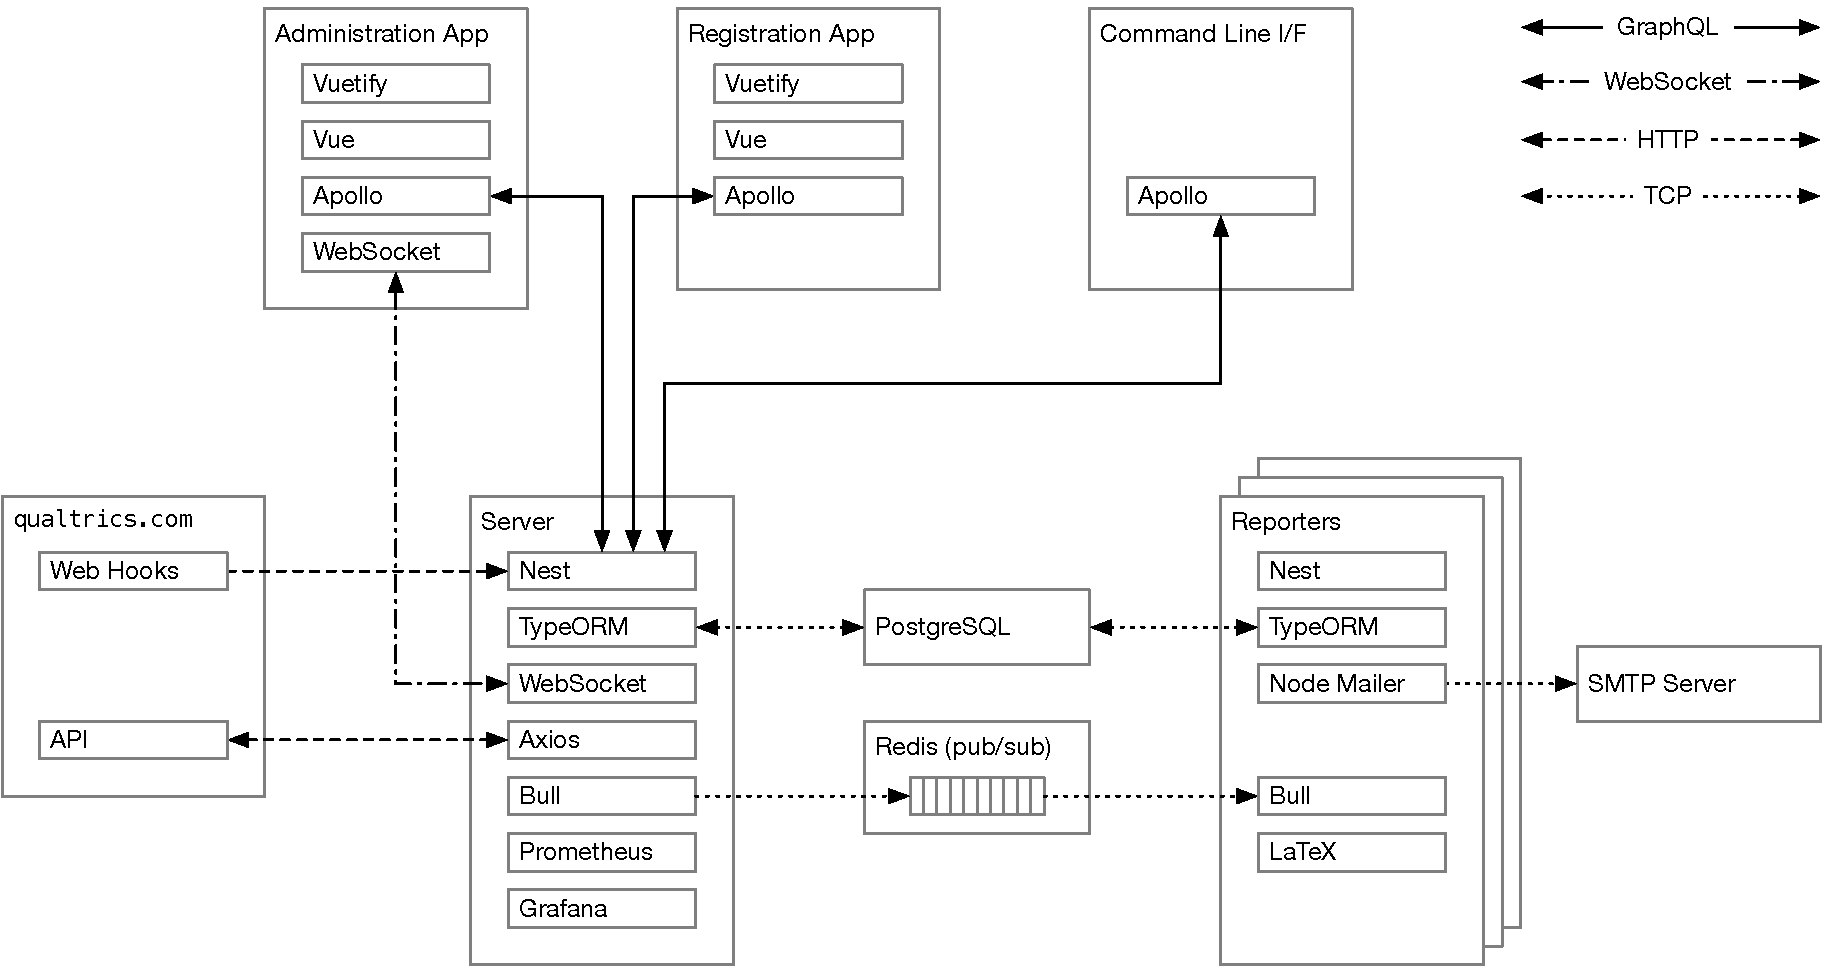
\includegraphics[width=\textwidth]{block-diagram}
  \caption{Block diagram of \caper.
    Communication between distributed processes is indicated in the legend.}
  \label{fig:block-diagram}
\end{figure}


\section{Deployment}
\label{sec:deployment}

\caper{} employs a fully-automated deployment
using \href{https://www.ansible.com/}{Ansible}.
The \ghsrc{ansible/provision.yaml}{provisioning file} contains commands for \gh{}, OS updates, etc.

\end{document}

%%% Local Variables:
%%% mode: latex
%%% TeX-master: t
%%% End:

% LocalWords:  Ansible ansible Qualtrics nd lr
